% !TeX root = ../../main.tex
% Add the above to each chapter to make compiling the PDF easier in some editors.

\section{Improvement In Time And IoU}\label{ord:ch5:sec1}

This section focuses of the variables annotation time $Time_{annot}$ and the precision measure $IoU$ from the benchmark measurements.
First, the relationship between time and user clicks is evaluated, to research this relationship in the terms of interactive segmentation methods.
Second, the variable $IoU$ is evaluated based on the four benchmark methods.
Third, the variable $Time_{annot}$ 

% TODO state number of samples per test

\subsection{Correlation Between Time And Clicks}\label{ord:ch5:sec1:subsec1}

% RE-1464 
In the following the relationship between time and user clicks and strokes is investigated, in order to promote the further analysis, which is strongly based on the annotation time $time_{annot}$. 
As introduced in Subsection \ref{ch2:sec3:eval_interactive_methods}, the common metric to measure the level of user interaction is the number of clicks $n_{clicks}$.
Thereby, $n_{clicks}$ functions as indicator for $time_{annot}$, which is the more meaningful variable in terms of ranking the amount of user interaction.
General, $n_{clicks}$ is not necessarily fair parameter, because the time per click may differ between various types of user interaction.

In the benchmark study the user interaction was recorded by the number of clicks $n_{clicks}$, number of strokes $n_{strokes}$, and the time $time_{strokes}$ required to perform the strokes.
The informative value of each single variable is limited, because either only clicks or strokes were used or both combined.
The stroke related variables are combined to the weighted strokes $ws$ by
\begin{equation} \label{equ:ws}
	ws = f_{stroke} * time_{strokes} + n_{strokes} 
\end{equation}
with the weighting factor $f_{stroke}=1.0$.
With $f_{stroke}=1.0$ it is estimated, that one second of stroking has the same value as one click.
In manual analysis of the data $f_{stroke}$ was determined, expecting a fair trade-off clicks and strokes.
To facilitate the comparison a single variable $cws$ is established by 
\begin{equation}
	cws = n_{clicks} + ws
\end{equation}
which combines clicks and strokes.

The relationship of the single variables is presented within a correlation matrix in Table \ref{tab:ch5:correlation-matrix}.
The reliability of the correlation matrix is supported by the size of the dataset with \getNumberBenchmarkAnnotations \space annotations.
% The calculated $\textnormal{\textit{p-value}} $ for the correlation table is always very low, except . 
%TODO ref that big dataset size and low p-value are 
% Correlation between time_{annot} and cws
The correlation between the time and weighted clicks and stroks $ corr \left(time_{annot}, cws \right) = 0.86341 $ is strong.
This confirms the relationship between these variables and supports their suitability for further evaluation.

Although, it should be noted that, the correlation value of $time_{annot}$ and $cws$ is not maximal.
This supports the thesis that $cws$ does not constitute a flawless representation of $time_{annot}$ and thereby is not a perfectly suitable performance measure.
However, $cws$ is still sufficient for the comparison of interactive methods, but the limitations have to be noted.
For the further evaluation mostly $time_{annot}$ will be used to represent the user interaction.

Last, attention should be drawn to the correlation between \gls{iou} and time \linebreak $ corr \left(time_{annot}, IoU \right) = 0.03808 $.
The low correlation indicates, that the a long annotation time not necessarily corresponds to a high \gls{iou}.
This may be caused by elaborate annotations of complicated objects, which require much time, but result in a comparable low $ IoU $.
Another reason is, that especially \gls{dl} methods can achieve a good IoU in little time, as discussed in Subsection \ref{ord:ch5:sec1:subsec3}.

% P-values support the reliability of the correlation matrix (except for correlatio between time and IoU) 

\begin{table}[h!]
	\centering
	\resizebox{\textwidth}{!}{
	\begin{tabular}{l|c c c c c c c}
		\toprule 		
							& $ time_{annot} $ & $ n_{clicks} $ & $ n_{strokes} $ & $ time_{strokes} $ & $ ws $ 	 & $ cws $  & $ IoU $ \\
		\midrule
		$ time_{annot} $	& 1 			 & 0.73251 		&  0.73184 		& 0.70028 		   & 0.74381 & 0.86341 &  0.03808 \\ 
		$ n_{clicks} $		& 0.73251		 & 1 			&  0.63629 		& 0.35356 		   & 0.46050 & 0.83002 &  0.03161 \\ 
		$ n_{strokes} $ 	& 0.73184 		 & 0.63629 		&  1 			& 0.78923		   & 0.98069 & 0.80735 & -0.00365 \\ 	
		$ time_{strokes} $ 	& 0.70028 		 & 0.35356	    &  0.78923	    & 1 			   & - & - & - \\ 
		$ ws $				& 0.74381 		 & 0.46050 		&  0.98069		& - & 1 & - & - \\ 
		$ cws $		  		& 0.86341 		 & 0.83002 		&  0.80735	    & - & - & 1 & - \\ 
		$ IoU $    			& 0.03808 		 & 0.03161		& -0.00365		& - & - & - & 1 \\ 								
		\bottomrule
	\end{tabular}}
	\caption[Correlation table]{
		Correlation table based on the \textit{Pearson} standard correlation coefficient \cite{Kirch08-CorrPearson}.
		The variables $ n_{clicks} $, $ n_{strokes} $, $ time_{strokes} $, and $ ws $ all show some correlation with $ time_{annot} $, while their combination $ cws $ shows a strong correlation. 
		The correlation between $ IoU $ and $ time_{annot} $ is almost not existent.
	}\label{tab:ch5:correlation-matrix}
\end{table}


\subsection{Analysis Of IoU}\label{ord:ch5:sec1:subsec2}

In the following the variable $IoU$ is evaluated in detail by the application of the statistical methods introduced in Section \ref{ord:ch2:sec4}.

% Limitation - The resulting mask was shown to the user, which may lead to futher editing resulting in a better IoU and more time
A limitation of the data received from the benchmark study, is that the resulting annotation mask was shown to the user and the editing are designed differently.
For the \gls{dextr} and \gls{iog} method the user interaction is more guided, while the interaction in the polygon and Watersheds method are designed more open.
The design difference in the editing process has perhaps led to the effect that for the latter methods, the user has continued to edit until a satisfactory \gls{iou} has been achieved.
Thereby, the annotations may have a similar \gls{iou}, but the time spent differs.
If the annotations had to be created in a certain time, the \gls{iou} would also be different, but it was deliberately decided against such a setup.

\subsubsection{Data Transformation}
Subsection \ref{ord:ch2:sec4:subsec1} already introduced the normality assumption for statistical methods as the Student's t-test and suggests a transformation of the data.
The histogram of the variable $IoU$ illustrates that the sample is not distributed normally as shown in Figure \ref{fig:ch5:sec1:data_raw}.
The data points are heavily skewed to the right. 
This is caused by many data points with a high \gls{iou} and comparatively few with a low \gls{iou}, produced by general good segmentation results.

In order to normalize the raw sample $ X_{raw} $, \cite{PS16-Statistics} suggests the logarithmic function
\begin{equation} \label{equ:trans_iou}
	X_{trans} = \frac{1}{2} * \log \left( \frac{1 + X_{raw}}{1 - X_{raw}}\right) 
\end{equation}
to transform the sample into $ X_{trans} $.
In Figure \ref{fig:ch5:sec1:data_transformed}, $ X_{trans} $ demonstrates the characteristics of a normal distribution.
Further the normality of $ X_{trans} $ is demonstrated by the probability plot shown in Figure \ref{fig:ch5:sec1:probplot}.

\begin{figure} [h]
	\centering
	\begin{subfigure}[t]{0.3\textwidth}
		\centering
		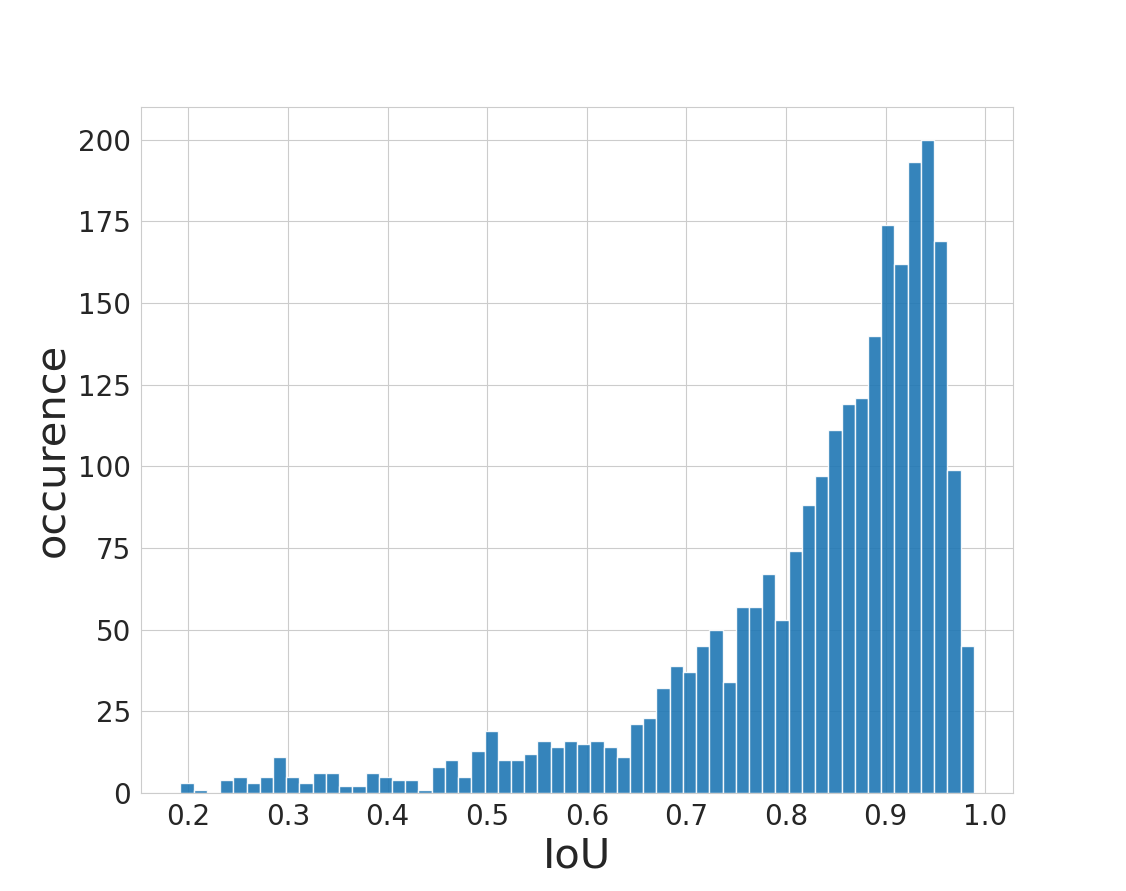
\includegraphics[width=\textwidth]{figures/chap51_iou_raw.png}
		\caption{
			Histogram of the $ IoU $ values as raw and unprocessed sample $ X_{raw} $.
		}\label{fig:ch5:sec1:data_raw}
	\end{subfigure}
	\hfill
	\begin{subfigure}[t]{0.3\textwidth}
		\centering
		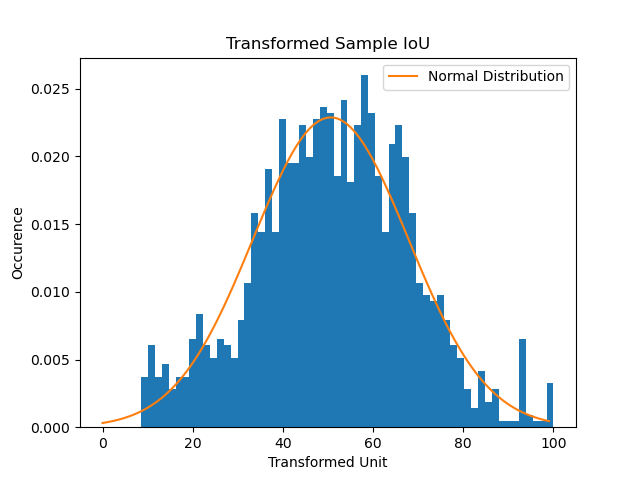
\includegraphics[width=\textwidth]{figures/chap51_iou_trans.png}
		\caption{
			Histogram of the transformed sample $ X_{trans} $ with a fitted normal distribution.
		} \label{fig:ch5:sec1:data_transformed}
	\end{subfigure}
	\hfill
	\begin{subfigure}[t]{0.3\textwidth}
		\centering
		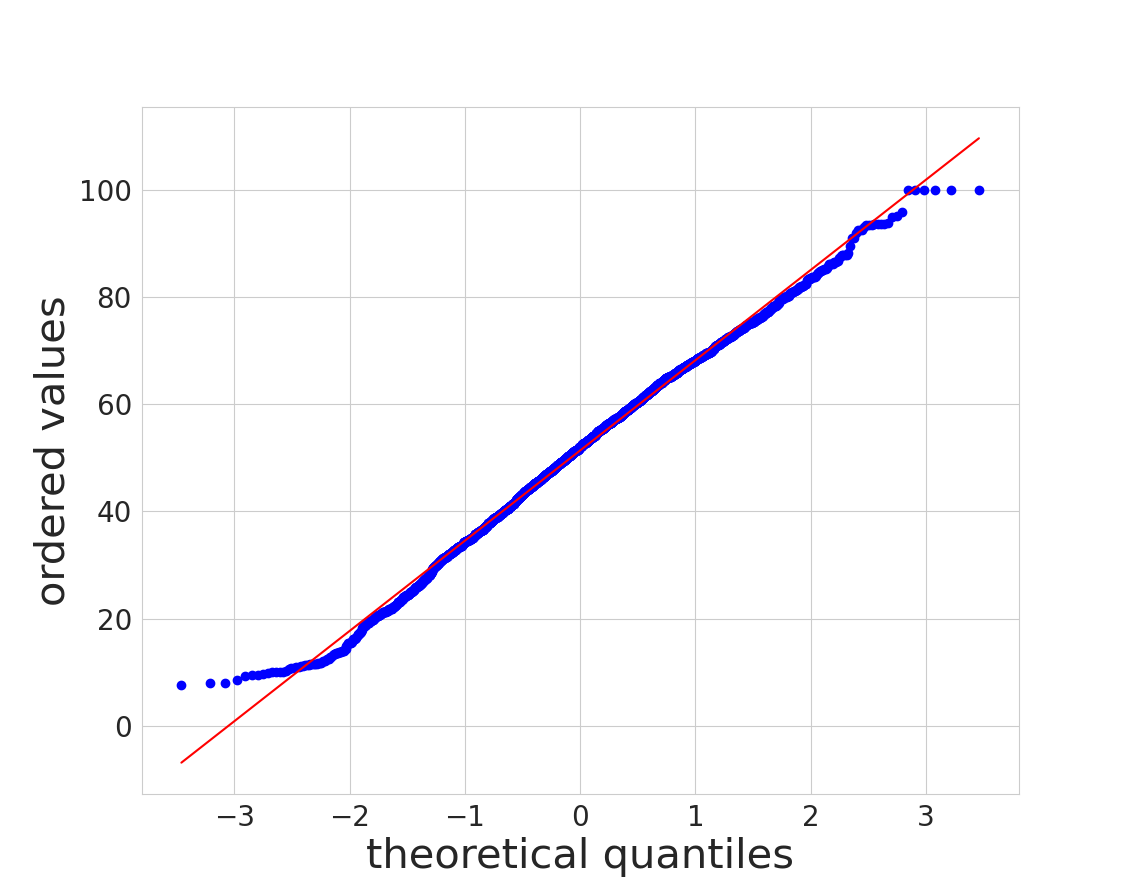
\includegraphics[width=\textwidth]{figures/chap51_iou_probplot.png}
		\caption{
			Normal probability plot of $ X_{trans} $.
		}\label{fig:ch5:sec1:probplot}
	\end{subfigure}
	\caption[IoU Sample Transformation]{		
		The sample $ X $ is transformed to achieve a normal distribution.
		As shown in a) $ X_{raw} $ is skewed to the right and not distributed normally.
		The transformation was performed by Equation \ref{equ:trans_iou}.
		The result of the transformation is $ X_{trans} $ and features normal characteristics, as illustrated in b) by the curve of the fitted normal distribution.
		In c) a normal probability plot confirms the normality in $ X_{trans} $.
	}\label{fig:ch5:sec1:data_transformation_iou}
\end{figure}


% Hypothesis testing
\subsubsection{Hypothesis Testing}

In the following multiple hypothesis tests are described, which divide the sample in two or four factors.

First, it is tested if \gls{dl} based methods (\gls{iog} and \gls{dextr}) are advantageous over classical methods (polygon drawing and watershed transformation).
This more general test results in the two factors $ IoU_{classical} $ and $ IoU_{dl} $.
Three different hypothesis tests are applied on these two factors.
Student's t-test evaluates the mean of the factors, Kruskal-Wallis the median of the factors, and Mann-Whitney the tendency of the factors as introduced in Subsection \ref{ord:ch2:sec4}.
The detailed settings and results of the tests are presented in Table \ref{tab:ch5:tests_on_iou}.
All three test come to the conclusion to accept $ H_{0} $, that in general the \gls{iou} of \gls{dl} based methods does not differ significantly from the \gls{iou} of classical methods.
The information value of this conclusion is especially strong, due to the application of three different tests with various null hypotheses.

\begin{table}[h!]
	\centering
	\resizebox{\textwidth}{!}{
	\begin{tabular}{l|c c c}
		\toprule 		
			 			& Student's t-test	& Kruskal-Wallis test 	& Mann-Whitney U-test \\
		\midrule
		data			& $ X_{trans} $		& $ X_{raw} $ 	 		& $ X_{raw} $ 	\\ 
		$H_{0}$			& $ \overline{IoU}_{classical} = \overline{IoU}_{dl} $ & $ med \left( IoU_{classical} \right)  = med \left( IoU_{dl} \right) $ & $ t_{dl} = t_{classical} $ 		\\
		$ H_{A} $		 	& $ \overline{IoU}_{classical} < \overline{IoU}_{dl} $ & $ med \left( IoU_{classical} \right) < med \left( IoU_{dl} \right) $ & $ ten \left( IoU_{dl} \right) \not= ten \left( IoU_{classical} \right) $ 	\\
		$ \alpha $		& $ 1\% $ 			& $ 1\% $ 		 		& $ 1\% $ 		\\ 	
		Statistic		& 0.0914 			& 786426	     		& 0.0711    	\\ 
		$ \textnormal{\textit{p-value}} $ 
						& 0.9272 			& 0.3949 		 		& 0.7898		\\ 
		$ H_{0} $		& accepted 			& accepted		 		& accepted 		\\
		\bottomrule
	\end{tabular}}
	\caption[Hypothesis Tests on $ IoU $]{
		Overview and results of the various statistical test performed on the variable $ IoU $.
		The variable $ IoU $ is evaluated by various values as the mean, median and tendency of the sample.
		Each factor contains 629 annotations.
		If the $ \textnormal{\textit{p-value}} $ is greater than the significance level $ \alpha $, $ H_{0} $ is accepted.
		The same result is achieved by all three different statistical tests, which supports its reliability.
	}\label{tab:ch5:tests_on_iou}	
\end{table}

% Kruskal-Wallis Test for four factors rejects H0.
Second, the variable $ IoU $ is evaluated in detail, thereby the Kruskal-Wallis test is applied using the four benchmark methods as factors.
The corresponding null hypothesis 
\begin{equation}
	H_{0}: med \left( IoU_{Polygon} \right) = med \left( IoU_{Watershed} \right) = med \left( IoU_{IOG} \right) = med \left( IoU_{DEXTR} \right)
\end{equation}
states, that the median values do not differ significantly at $ \alpha=1\% $.
$ H_{A} $ assumes that $ H_{0} $ is not true, but does not define which factor is different.
As result the statistic returns $ \textnormal{\textit{p-value}} = 0.0015 $, therefore $ H_{0} $ is rejected and $ H_{A} $ accepted.

It can be determined what factors differ significantly, by the application of the DSCFs  test \cite{CF91-dscf}.
In this test it is shown that, $ med \left( IoU_{DEXTR} \right) $ is greater, while $ med \left( IoU_{IOG} \right) $ is lower than the other factors. 
In Figure \ref{fig:ch5:sec1:iou_box_plot} this may seems like a small difference, but the statistical relevance is confirmed.
Conspicuous in the plot shown are the high amount of outliers and the wide range of the lower quarter of the box plot.
An explanation for this are demanding annotations from the domain anomaly or the failure of the methods on single annotations.
The number of outliers may seem large, but must be put in proportion to the size of the data with \getNumberBenchmarkAnnotations \space annotations.

\begin{figure}
	\centering
	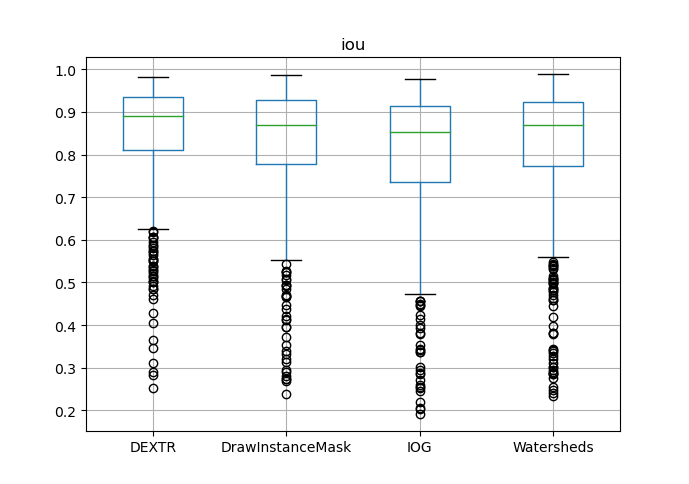
\includegraphics[width=0.9\textwidth]{figures/chap51_boxplot_iou.png}
	\caption[Box plot IoU per method]{
		Box plot of the variable $ IoU $ for the four benchmark methods.
		$ med \left( IoU_{DEXTR} \right) $ is superior over the other factors, while $ med \left( IoU_{IOG} \right) $ performs worst.
		The classical methods to not differ significantly in their median values $ med \left( IoU_{Polygon} \right) $ and $ med \left( IoU_{Polygon} \right) $.
	} \label{fig:ch5:sec1:iou_box_plot}
\end{figure}
% TODO sort the box plot by method types -> Polygon, Watershed, DEXTR, IOG



\subsection{Analysis Of Time}\label{ord:ch5:sec1:subsec3}
% RE-1466
Now the variable $Time_{annot}$ is evaluated, the evaluation procedure is analog to the previous evaluation of the variable $IoU$.
\subsubsection{Data Transformation}

The histogram of the raw sample for the variable $Time_{annot}$ does not fit a normal distribution as shown in Figure \ref{fig:ch5:sec1:time_raw}.
Instead, the data points are heavily skewed to the left, because $Time_{annot}$ is usually short, but can also be larger.
\cite{PS16-Statistics} suggests to transform the sample by the logarithmic function 
\begin{equation} \label{equ:trans_time}
	X_{trans} = \log \left( X_{raw} \right) 
\end{equation}
to adapt the shape of a normal distribution, $X_{trans}$ is shown in Figure \ref{fig:ch5:sec1:time_transformed}.
$X_{trans}$ is similar to a normal distribution, which is also supported by the corresponding normal probability plot illustrated in Figure \ref{fig:ch5:sec1:time_probplot}

\begin{figure} [h]
	\centering
	\begin{subfigure}[t]{0.3\textwidth}
		\centering
		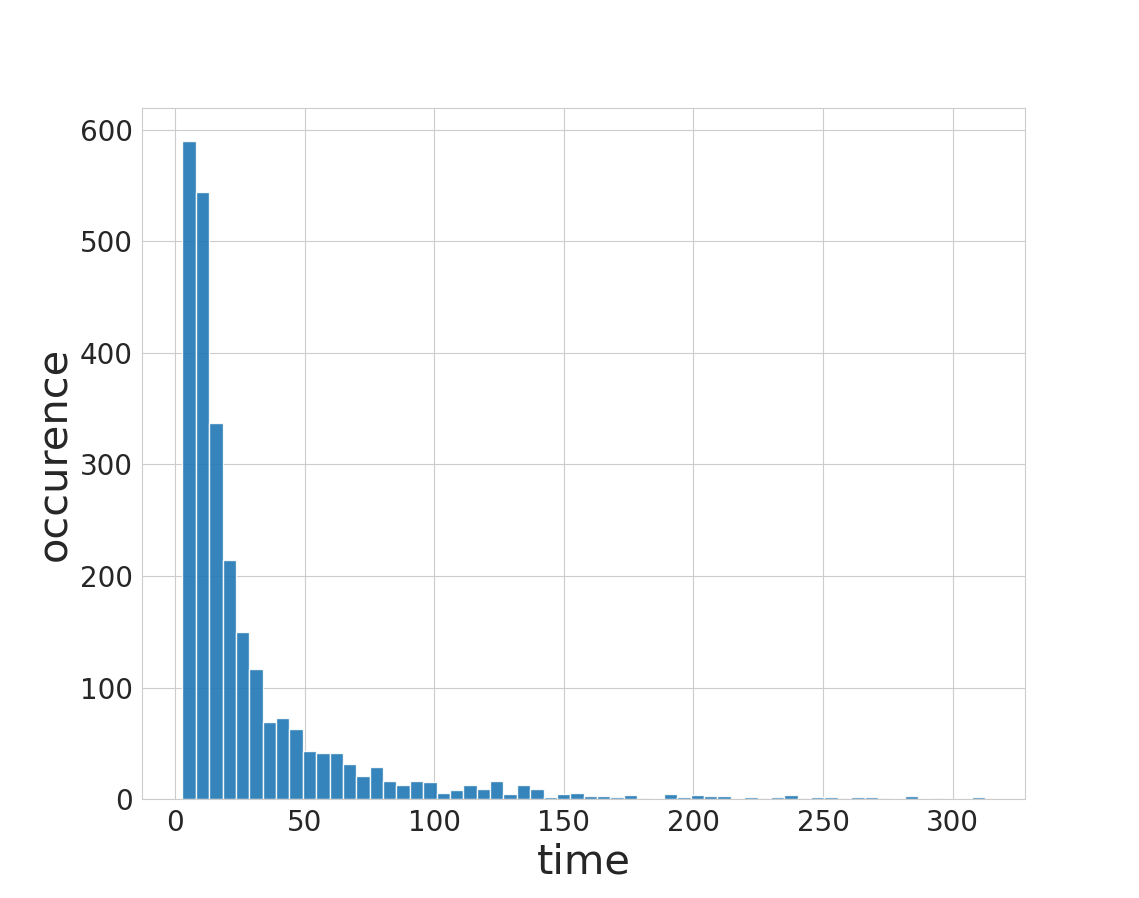
\includegraphics[width=\textwidth]{figures/chap51_time_raw.png}
		\caption{
			$Time_{Annot}$ as raw and unprocessed sample $X_{raw}$.
		}\label{fig:ch5:sec1:time_raw}
	\end{subfigure}
	\hfill
	\begin{subfigure}[t]{0.3\textwidth}
		\centering
		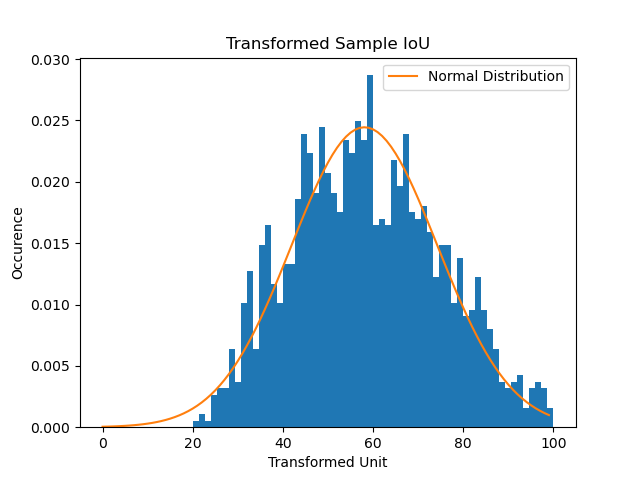
\includegraphics[width=\textwidth]{figures/chap51_time_trans.png}
		\caption{
			Transformed sample $X_{trans}$ with fitted normal distribution.
		} \label{fig:ch5:sec1:time_transformed}
	\end{subfigure}
	\hfill
	\begin{subfigure}[t]{0.3\textwidth}
		\centering
		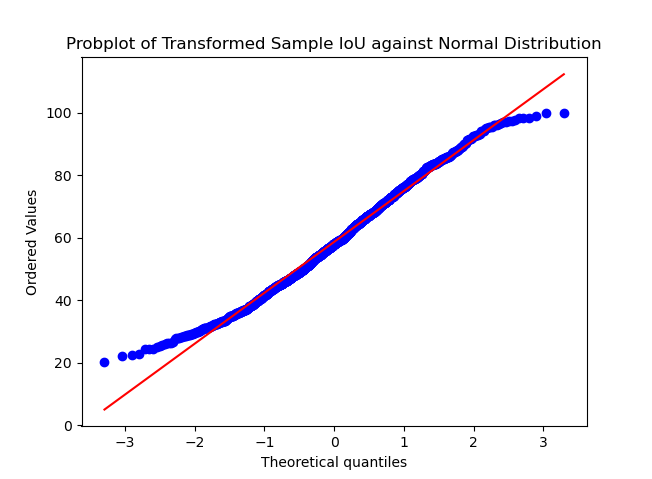
\includegraphics[width=\textwidth]{figures/chap51_time_probplot.png}
		\caption{
			Normal Probability Plot of $X_{trans}$.
		}\label{fig:ch5:sec1:time_probplot}
	\end{subfigure}
	\caption[Time Sample Transformation]{
		Transformation of the sample to achieve a normal distribution.
		In a) $X_{raw}$ is shown, which is skewed to the left and not normally distributed.
		The sample is transformed by Equation \ref{equ:trans_time}.
		The result is $X_{trans}$ now shows normal characteristics, as illustrated by the curve of the fitted normal distribution in b).
		The corresponding normal probability plot of $X_{trans}$ is shown in c), which confrims the normal characteristics of $X_{trans}$.
	}\label{fig:ch5:sec1:time_transformation_iou}
\end{figure}




\subsubsection{Hypothesis Testing}

The setting for this hypothesis testing is analog to the previous tests on $IoU$.
In further evaluation the variable $time_{annot}$ is referred to as $time$, in order to enable a simple distinction between the factors.

First, more general tests are applied on the factors $time_{classical}$ and $time_{dl}$.
The Student's t-test, Kruskal-Wallis test, and Mann-Whitney are performed and their details are presented in Table \ref{tab:ch5:tests_on_time}.
All three tests come to the conclusion to reject $H_{0}$ and accept $H_{A}$.
This proves that the annotation time of \gls{dl} based methods is significantly faster than the annotation time of classical methods, as also illustrated in Figure \ref{fig:ch5:sec1:time_box_plot}.
The information value of this conclusion is especially expressive, due to the application of three different tests with various null hypotheses.

\begin{table}[h!]
	\centering
	\resizebox{\textwidth}{!}{
	\begin{tabular}{l|c c c}
		\toprule 		
		& Student's t-test	& Kruskal-Wallis test 	& Mann-Whitney U-test \\
		\midrule
		data			& $X_{trans}$		& $X_{raw}$ 	 		& $X_{raw}$ 	\\ 
		$H_{0}$			& $\overline{time}_{classical} = \overline{time}_{dl}$ & $med \left( time_{classical} \right)  = med \left( time_{dl} \right)$ & $ten \left( time_{dl} \right) = ten \left( time_{classical} \right)$ 		\\
		$H_{A}$		 	& $\overline{time}_{classical} > \overline{time}_{dl}$ & $med \left( time_{classical} \right) > med \left( time_{dl} \right) $ & $ten \left( time_{dl} \right) \not= ten \left( time_{classical}\right) $ 	\\
		$\alpha$		& $1\%$ 			& $1\%$ 		 		& $1\%$ 		\\ 	
		Statistic		& 29.2979			& 332052	     		& 635.327    	\\ 
		$\textnormal{\textit{p-value}}$ 
		& $1.3 * 10^{-159}$		& $1.7 * 10^{-140}$ 		 		& $3.4 * 10^{-140}$ 		\\ 
		$H_{0}$		  	& rejected 			& rejected		 		& rejected 		\\
		\bottomrule
	\end{tabular}}
	\caption[Hypothesis Tests on $time$]{
		Overview and results of the various statistical test performed on the variable $time$.
		The variable $time$ is evaluated by various values as the mean, median and tendency of the sample.
		Each factor contains 629 annotations.
		If the $\textnormal{\textit{p-value}}$ is lower than the significance level $\alpha$, $H_{0}$ is rejected and $H_{A}$ is accepted.
		The same result is achieved by all three different statistical tests, which supports its reliability.
	}\label{tab:ch5:tests_on_time}
\end{table}
%TODO Mann-Whitney U-test - as one sided test - in which direction goes the smaller or greater sign.
% Kruskal-Wallis Test for four factors rejects H0.
Second, the variable $time$ is evaluated for the four benchmark methods by the Kruskal-Wallis test.
The null hypothesis 
\begin{equation}
	H_{0}: med \left( time_{Polygon} \right) = med \left( time_{Watershed} \right) = med \left( time_{IOG} \right) = med \left( time_{DEXTR} \right)
\end{equation}
assumes, that the median values do not differ significantly at $\alpha=1\%$.
$H_{A}$ states that $H_{0}$ is not true.
The statistic returns $\textnormal{\textit{p-value}}=2.7*10^{-143}$, as a result $H_{0}$ is rejected and $H_{A}$ accepted.

Based on the post analysis by the DSCF test \cite{CF91-dscf}, the factors polygon and Watershed do not differ significantly.
In contrast, the difference between $med \left( time_{DEXTR} \right)$ and $med \left( time_{IOG} \right)$ may be titled significant.

The differences between the factors are illustrated in Figure \ref{fig:ch5:sec1:time_box_plot}.
The \gls{iog} and \gls{dextr} method clearly demonstrate a lower annotation time than the polygon and Watersheds method.
It is extraordinary to note that for all methods the last quarter of the box plot covers a larger area than the first quarter.
One possible reason is that the different participants spent different amounts of time on particularly complicated objects.
Notable, is that this effect is extreme for the polygon and Watershed method, where approximately one quarter spent more than 60 seconds respectively 50 seconds on one annotation. 
This is perhaps caused, due to the possibility for editing is designed more open for these methods and therefore more time was spent on editing with these these methods, as mentioned at the beginning of this Section.

\begin{figure}
	\centering
	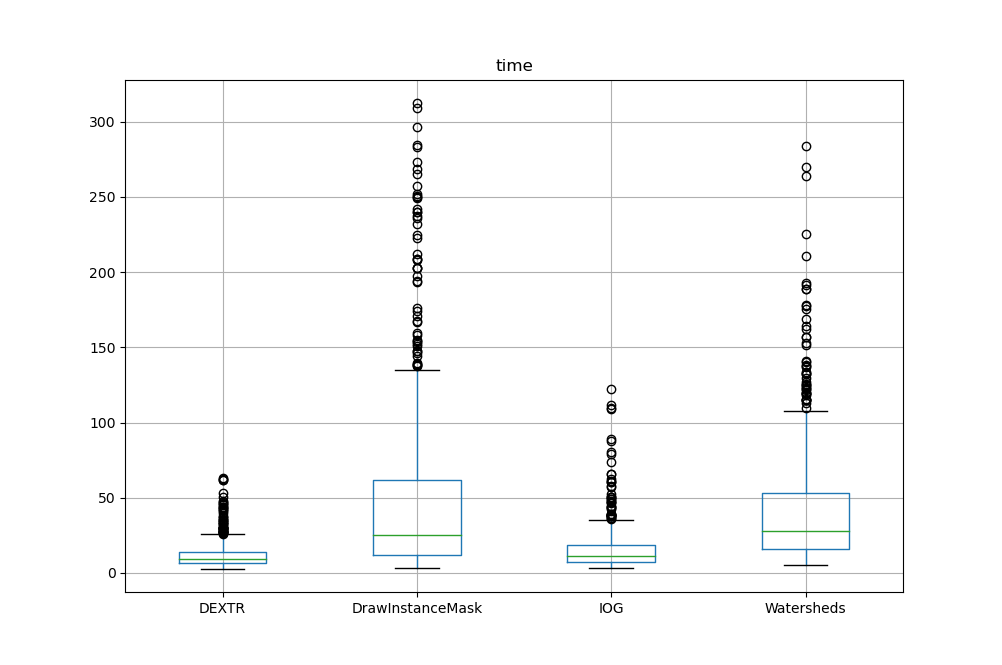
\includegraphics[width=0.9\textwidth]{figures/chap51_time_boxplot.png}
	\caption[Box plot IoU per method]{
		Box plot of the variable $ time $ for the four benchmark methods.
		It can be seen clearly, that $ med \left( time_{DEXTR} \right) $ and $ med \left( time_{IOG} \right) $ are lower than $ med \left( time_{Polygon} \right) $ and $ med \left( time_{Polygon} \right) $.
		In general, the polygon and Watersheds method require a longer annotation time, where the last quarter of the box plot covers a relatively wide range with many outliers. 
		%Despite the difference
	} \label{fig:ch5:sec1:time_box_plot}
\end{figure}
% TODO sort the box plot by method types -> Polygon, Watershed, DEXTR, IOG



Combining the results of the evaluation from $ IoU $ and the $ time_{annot} $, it can be said that all methods may achieve an approximately the same level of accuracy.
But the difference between the two types of methods is that, \gls{dl} based method require significantly less time to achieve this state of \gls{iou}.




